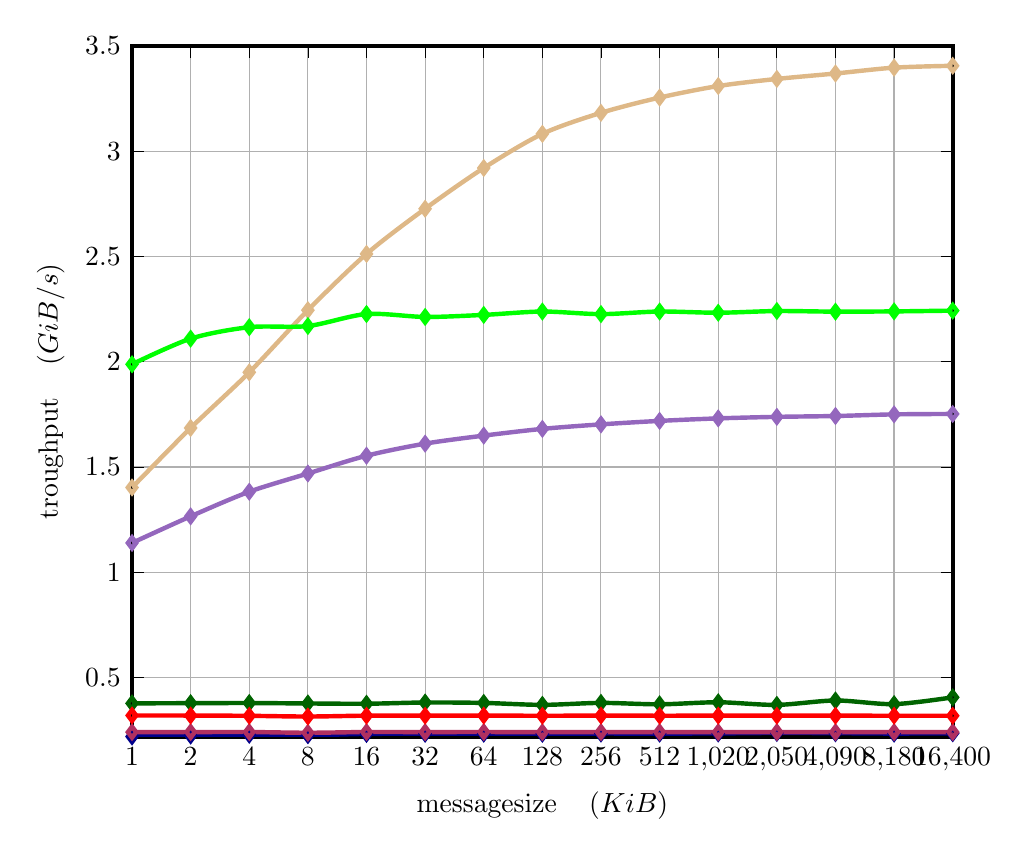
\begin{tikzpicture}
\pgfplotsset{every axis/.append style={ultra thick},compat=1.5}
\definecolor{mycolor0}{rgb}{0.00000, 0.39216, 0.00000}
\definecolor{mycolor1}{rgb}{0.00000, 0.00000, 0.54510}
\definecolor{mycolor2}{rgb}{0.69020, 0.18824, 0.37647}
\definecolor{mycolor3}{rgb}{1.00000, 0.00000, 0.00000}
\definecolor{mycolor4}{rgb}{0.58039, 0.40392, 0.74118}
\definecolor{mycolor5}{rgb}{0.87059, 0.72157, 0.52941}
\definecolor{mycolor6}{rgb}{0.00000, 1.00000, 0.00000}
\definecolor{mycolor7}{rgb}{0.00000, 1.00000, 1.00000}
\definecolor{mycolor8}{rgb}{1.00000, 0.00000, 1.00000}
\definecolor{mycolor9}{rgb}{0.39216, 0.58431, 0.92941}
    \begin{axis}[
        xlabel=$\mathrm{message size}\quad\left(KiB\right)$,
        ylabel=$\mathrm{troughput}\quad\left(GiB/s\right)$,
        width=0.99*\textwidth,
        xmajorgrids,
        enlargelimits=false,
        scaled ticks=true,
        ymajorgrids,
        log basis x=2,
        xmode=log,
		ymax=3.5,
        log ticks with fixed point,
        x tick style={color=black},
        y tick style={color=black},
        x grid style={white!69.01960784313725!black},
        y grid style={white!69.01960784313725!black},
]
\addplot[
        smooth,
        mark=diamond,
        color=mycolor0,
    ] plot coordinates {
            (1,0.37756)
        (2,0.37854)
        (4,0.37922)
        (8,0.37711)
        (16,0.37580)
        (32,0.38171)
        (64,0.37966)
        (128,0.37049)
        (256,0.37985)
        (512,0.37309)
        (1024,0.38283)
        (2048,0.37037)
        (4096,0.39125)
        (8192,0.37393)
        (16384,0.40623)

    };
    \addplot[
        smooth,
        mark=diamond,
        color=mycolor1,
    ] plot coordinates {
            (1,0.22011)
        (2,0.22487)
        (4,0.22856)
        (8,0.22639)
        (16,0.23260)
        (32,0.23339)
        (64,0.23379)
        (128,0.23338)
        (256,0.23435)
        (512,0.23402)
        (1024,0.23483)
        (2048,0.23715)
        (4096,0.23608)
        (8192,0.23414)
        (16384,0.23565)

    };
    \addplot[
        smooth,
        mark=diamond,
        color=mycolor2,
    ] plot coordinates {
            (1,0.24103)
        (2,0.24122)
        (4,0.24149)
        (8,0.23800)
        (16,0.24146)
        (32,0.24127)
        (64,0.24155)
        (128,0.24085)
        (256,0.24130)
        (512,0.24131)
        (1024,0.24115)
        (2048,0.24130)
        (4096,0.24115)
        (8192,0.24120)
        (16384,0.24118)

    };
    \addplot[
        smooth,
        mark=diamond,
        color=mycolor3,
    ] plot coordinates {
            (1,0.32011)
        (2,0.31972)
        (4,0.31844)
        (8,0.31509)
        (16,0.31922)
        (32,0.31916)
        (64,0.31962)
        (128,0.31873)
        (256,0.31950)
        (512,0.31892)
        (1024,0.31921)
        (2048,0.31918)
        (4096,0.31903)
        (8192,0.31891)
        (16384,0.31873)

    };
    \addplot[
        smooth,
        mark=diamond,
        color=mycolor4,
    ] plot coordinates {
            (1,1.13937)
        (2,1.26570)
        (4,1.38249)
        (8,1.46911)
        (16,1.55358)
        (32,1.61096)
        (64,1.64898)
        (128,1.68102)
        (256,1.70240)
        (512,1.71890)
        (1024,1.73087)
        (2048,1.73808)
        (4096,1.74211)
        (8192,1.74987)
        (16384,1.75194)

    };
    \addplot[
        smooth,
        mark=diamond,
        color=mycolor5,
    ] plot coordinates {
            (1,1.40260)
        (2,1.68528)
        (4,1.94953)
        (8,2.24462)
        (16,2.51169)
        (32,2.72636)
        (64,2.91972)
        (128,3.08186)
        (256,3.18175)
        (512,3.25419)
        (1024,3.30899)
        (2048,3.34268)
        (4096,3.36851)
        (8192,3.39623)
        (16384,3.40511)

    };
    \addplot[
        smooth,
        mark=diamond,
        color=mycolor6,
    ] plot coordinates {
            (1,1.98774)
        (2,2.10942)
        (4,2.16385)
        (8,2.16933)
        (16,2.22630)
        (32,2.21246)
        (64,2.22224)
        (128,2.23820)
        (256,2.22587)
        (512,2.23826)
        (1024,2.23248)
        (2048,2.24059)
        (4096,2.23763)
        (8192,2.23890)
        (16384,2.24246)

    };
     
    \end{axis}
    \end{tikzpicture}       
    